\documentclass[a4paper]{article}

%% Language and font encodings
\usepackage[english]{babel}
\usepackage[utf8x]{inputenc}
\usepackage[T1]{fontenc}


%% Sets page size and margins
\usepackage[a4paper,top=3cm,bottom=2cm,left=3cm,right=3cm,marginparwidth=1.75cm]{geometry}

%% Useful packages
\usepackage{ amssymb }
\usepackage{amsmath}
\usepackage{graphicx}
\usepackage[colorinlistoftodos]{todonotes}
\usepackage[colorlinks=true, allcolors=blue]{hyperref}
\usepackage{bm}
\setcounter{tocdepth}{2} 

\title{Literature Study}
\author{You}

\begin{document}
\maketitle
\newpage
\tableofcontents
\newpage
\begin{abstract}
Your abstract.
\end{abstract}
\newpage
\section{Literature Study}
\subsection{Neural networks}
Artificial neural networks (ANN) were first described in 1943 By Warren McCulloch and Walter Pitts in an attempt to provide a usable mathematical model based on neurons firing in the brains \cite{Pitts43}. But at the time most researchers found little use for them as there wasn't enough computing power to make effective use of ANN. More recently thanks to the increase in availability of computational power and advancements in techniques used in ANN, they are again at the center of attention. 

The goal of an ANN is to classify given inputs under their corresponding labels. The labels are known during training and the variables are changed in such a way that it maximizes the chance for the ANN to predict the correct label corresponding to an input. Then when the network is deemed to be optimized it can be used to predict the labels for inputs it has never seen before and hopefully predict them correctly.

\subsubsection{Basic architecture}
A neural network consists of a number of layers, with each layer containing a number of units and connections run from these units to other units. In their basic form the network starts with an input layer wich connects to the inputs and from then on the units in each layer connect vertically to higher-up layers that are closer to the final layer, the output layer. If these connections are one-way this type of ANN is also known as a feed-forward neural network. All the layers in between the input and output layers are known as the hidden layers. Because from an outside perspective the ouputs of these layers are not visible.

In each unit a simple operation is performed on the inputs. 
\begin{equation}
y = \mathit{f}(WX + b)
\end{equation}
The output $y$ is a function of the input $X$ and 2 "trainable" variables $W$,the weights, and $b$, the bias. The weights consist of a matrix of values with the number of columns equal to the inputs and number of rows equal to the outputs. The function $\mathit{f}$ is called the activation function. This can be just a basic linear operation or in a lot of cases a non-linear function. This is where neural etworks get their strength in working as classifiers. Becaus they can contain non-linear functions they can be suprisingly good at mimicing and predicting real patterns. In figure \ref{fig:graves}, six commonly used activation functions are shown.


\begin{figure}
  \centering
      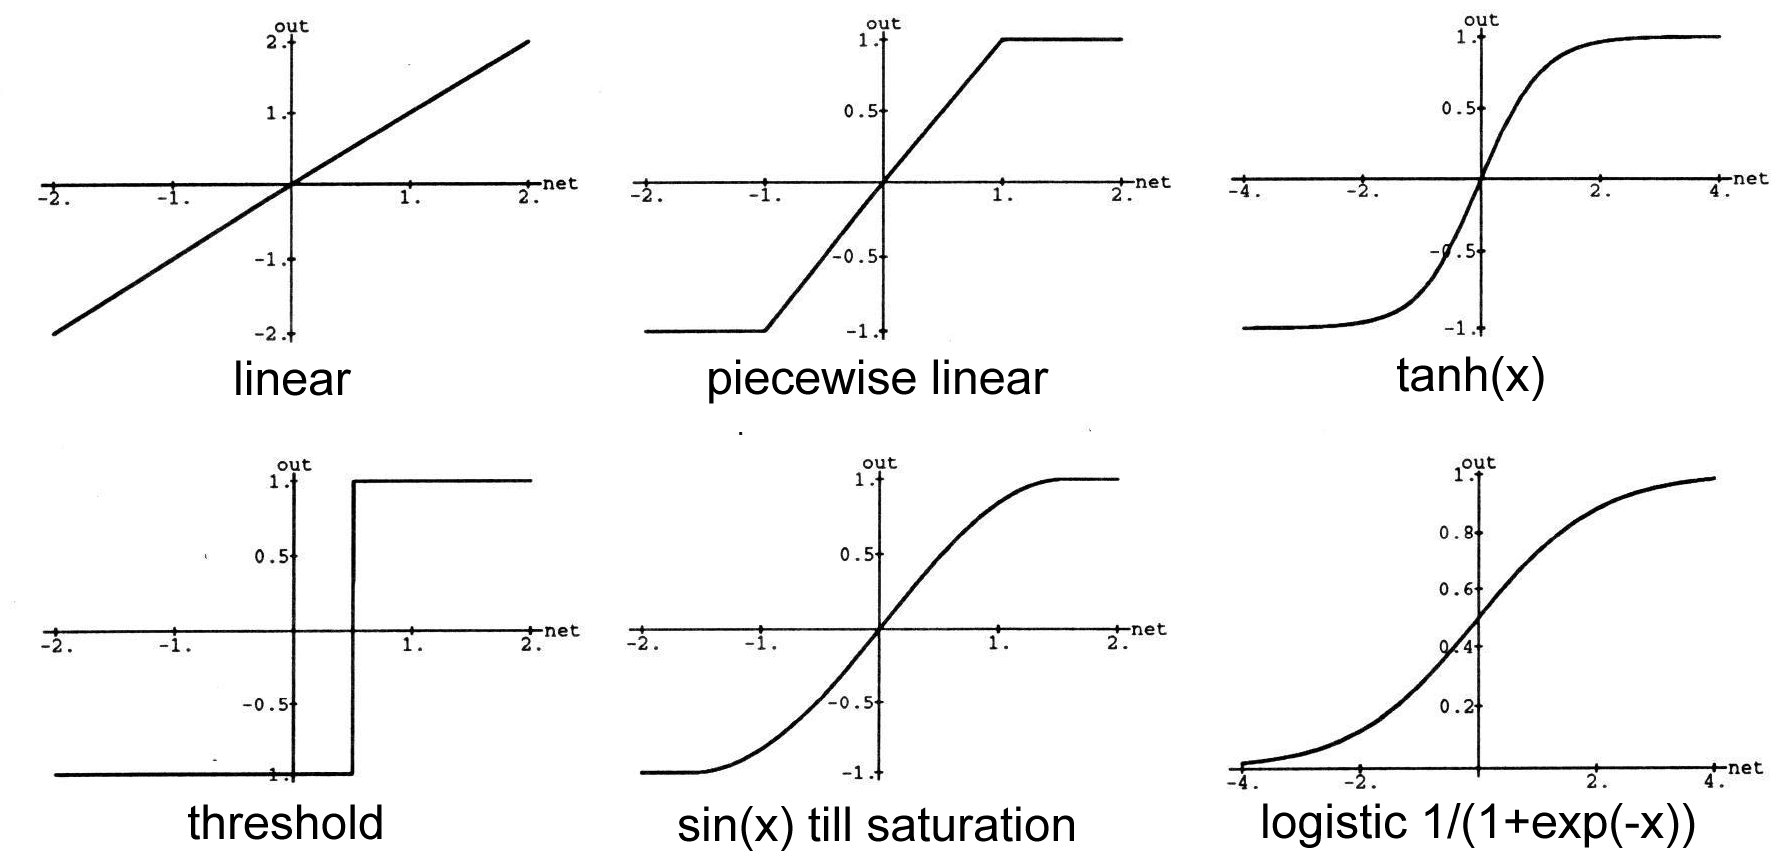
\includegraphics[width=0.5\textwidth]{test.png}
  \caption{Activation functions[\cite{Graves},page 14}
  \label{fig:graves}
\end{figure}

In a non-linear layer a non-linear function is applied to the inputs. There's a variety of different functions that are used. The most common ones are the sigmoid 
\begin{equation}
\sigma(x) = frac{1}{1+e^{-x}}
\end{equation}
 and the $\tanh$ functions. They are related by the simple linear transform.
\begin{equation}
\tanh(x) = 2\sigma(2x)-1
\end{equation}

After we get the final output vector we must transform it first in a way that makes it easier to detrmine what is the most likely output. First the labels are "one-hot" encoded. This means that for each label a vector is created with a single 1 and the rest of the vector zeroes. For example $a$ has a 1 on the first position, $b$ has a 1 on the second position etc... Now the final output vector has to be transformed so that it assigns a probability rating to each possible label for the input. For this a softmax function is used.
\begin{equation}
S(y_i) = \frac{e^{y_i}}{\sum\limits_j e^{y_j}}
\end{equation}
Now every label has a probability rating but to be able to use this rating to train the neural network a loss has to be calculated. There are multiple types of loss functions but the most used one is the cross-entropy-loss. 
\begin{equation}
\mathcal{L} (S,L) = -\sum\limits_i L_i\log(S_i)
\end{equation}
Here $S$ is the final output after the softmax function and L is the vector containing the one-hot encoded labels. 




\subsubsection{Recurrent Neural Networks}
The previously discussed nerual networks only contain connections that go up to a higher numbered layer. With this type of architecture it is impossible for the network to know what is happening in the units to the right or left of it. In a more practical sense it means that a network has no memory of previous inputs and no knowledge of future inputs. In speech however it is often important to know which letters were previously said to be able to make a good guess on which letters you're hearing now. RNN's are an attempted answer to this. In essence a RNNadds extra connections in a single layer. All the added connections thus go are horizontal. These can be one way or they can go both ways, depending on what is required for the task. In the figure it can be seen that a connection to the right means that $y_t$ depends as well on $y_{t-1}$ and a connection to the left means that $y_{t-1}$ depends on $y_{t}$. The introduction of an RNN thus gives the neural network some form of memory which can be very useful for speech applications.

Now in every unit the operation performed on the inputs looks a bit different.
\begin{equation}
y = \mathit{f}(W_iX + b_i + W_hy^{t-1} + b_h)
\end{equation}
Here $W_h$ are the weights for the output of the unit at the previous timestep $y^{t-1}$ and $b_h$ is the bias added to it. To calculate the output one now starts at timestep $t=1$ and then increments $t$ until the final unit is reached. $y^{0}$ has to be chosen for each unit wich corresponds to the starting state of the neural network.


One of the problems with training RNN is known as the vanishing gradient problem. It was identified by Hochreiter in [insert hochreiter thesis here] as a consequence of backpropagation. In practice it means that a RNN forgets about information that happened too long in the past. Since backpropagation computes gradients using the chain rule. In an $n$ layer network $n$ of these small numbers have to be multiplied to get to the gradient of the first layer. The opposite of this, called the exploding gradient can also happen but is often easily remedied by limiting the gradient to a maximum value. To solve the vanishing gradient in RNN Hochreiter introduced LSTM[insert 1999 paper].

\subsubsection{long short term memory}
The basic architecture for long short-term memory (LSTM) looks very similar to that of the memory cell of a computer. There is a read port, a write port and an erase port. These allow to memory cell to decide when it wants to read data, write data or erase data, by putting the respective variable for a port to $1$ to open the port and to $0$ to close the port. But whilst in a computer architecture those are binary decisions. In the case of ANN neural network they are continuous differentiable functions going from $0$ to $1$. This allows the gradient to be calculated via backpropagation. 
In the LSTM cell we speak of the input gate, the output gate and the memory gate. They are generally referred to as $\bm{i}$,$\bm{o}$ and 
$\bm{f}$. An lstm cell also has a state which is normally referred to as $\bm{c}_t$ but will be referred to as $\bm{s}$ here to not be confused with the context vector of the LAS network. They are defined as follows \cite{RNN}, page 5

\begin{equation}
i_t = \sigma(W_{xi}x_t + W_{hi}h_{t-1} + W_{ci}c_{t-1} + b_i)
\end{equation}

\begin{equation}
f_t = \sigma(W_{xf}x_t + W_{hf}h_{t-1} + W_{cf}c_{t-1} + b_f)
\end{equation}

\begin{equation}
c_t = f_tc_{t-1} + i_t\tanh(W_{xc}x_t + W_{hc}h_{t-1} + b_c)
\end{equation}
\begin{equation}
o_t = \sigma(W_{xo}x_t + W_{ho}h_{t-1} + W_{co}c_{t-1} + b_o)
\end{equation}
\begin{equation}
h_t = o_t \tanh(c_t)
\end{equation}

\subsubsection{training}
With the loss function we can now begin training the neural network. First though the inputs are split into 3 different groups. A train,test and validation group. The train set is the biggest and is the basic set of inputs during training. Where each iteration the loss is calculated for a batch of the train set. The validation set exists to prevent overfitting. Overfitting happens when the ANN learns to recognize only his given inputs and starts to perform worse on new inputs that he hasn't seen yet. So to mimic this, part of the training data is seperated and after a certain number of iterations the loss of the validation set is calculated. If this is higher than the loss of the previous time there is a chance of overfitting and it might be time to stop training if this happens multiple times in a row. The test set is an extra overfitting measure. After multiple revisions of the hyperparameters of the model, like the sie of the layers or the amount of layers. It's possible to begin overfitting on the validation set the test set can be used as a final check, but it can only be used after training is completely finished.




 
\subsection{Learning}
To be able to use an ANN it has to be trained properly. There are different ways of learning that can be used. Where the biggest difference between them is the type of cost function applied to the outputs. In \textit{supervised learning} the outputs of the neural network are compared against the desired values of the outputs for the given inputs. Two other types of learning are \textit{unsupervised learning} and \textit{reinforcement learning}, both do not have a specific input-output mapping. The former instead looks for structures or possibly porbability distributions over the data, whilst the latter provides information about the wether the outputs are good or bad, without specifying the desired values.\cite{Bish}
\subsection{multi task learning}
Multi task learning is an inductive transfer mechanic that allows a neural network to be trained in parallel to perform multiple relatable tasks whilst keeping the representation shared.

There are a variety of benefits to multi task learning. Which i will sum up in the next few sections.

\subsubsection{Eavesdropping}

Eavesdropping occurs when the hidden features $F$ of a given task $T$ are shared by another task $T'$. If these hidden featres are difficult to learn for task $T$ and easier to learn for task $T'$, $T$ can eavesdrop on the shared hidden layer to help itself learn $F$.
\subsubsection{Data amplification}
Data amplification is an increase in the availability of data thanks to MTL. There are a variety of different ways this can be of benefit. Statistical data sampling occurs when a task $T$ has been corrupted by noise and a relatable task $T'$ that shares some of the same features of $T$ has been corrupted by a different noise source. If the network would be trained only on $T$ it woulb be possible to overfit on the noise source but if both tasks were used in MTL. The network would focus more on making an accurate representation of the shared features.
Sampling data amplification is very similar to statistical amplification but now it occurs when there is no noise present in the tasks. If two tasks $T$ and $T'$ consist out of shared and non-shared features like this:
$$T(i)  = F(i) + G(i)$$
$$T'(i) = F(i) + H(i)$$
Training them in parallel helps to provide the neural net more information about the hidden feaures $F$ that are shared by both. This is especially usefull in cases when there is little training data available for a specific task. Also if we consider for example the case where $T'(i) = F(i)$ it is quite obvious that it would be useful for a net to be trained simultaneously on $T$ and $T'$ as it would help the network gain a correct representation of $F$ unperturbed by any other features 
\subsubsection{Attribute selection}
If there are two tasks $T$ and $T'$ that both share a feature $F$. Suppose now that $F$ uses only a small number of the total inputs. A neural net only training on $T$ will have a lot of difficulty finding the relevant inputs for $F$, if there is a lot of noise on the data. If both $T$ and $T'$ are being learned at the same Data amplification will help to find the relevant inputs that affect $F$.
\subsubsection{Representation Bias}
Because ANN are initialized with random weights optimizing the same net for the same task $T$ multiple times, will rarely result in an identical net. If we consider the complete set on all nets trained on this task $T$, some of these nets will regularize better because they better represent the domain's regularities. If we another task $T'$ that shares one of these regularities,$F$. If we train the net on both $T$ and $T'$ the net will be biased towards a representation of the regularity $F$ near the intersections between $T$ and $T'$ and have a bigger chance of forming a better regularization.
\subsubsection{Overfitting prevention}
Suppose two tasks $T$ and $T'$ both share feature $F$. Suppose $T$ has come to the point where it would begin to overfit on $F$ if it were trained alone. Training on $T'$ helps the net in two ways.
Firstly consider the case that $T'$ has not begun to overfit on $F$ then $T'$ provides a gradient that will push $F$ towards a better model instead of an overfitted one.
In the second case both $T$ and $T'$ use $F$ in different ways. Suppose $T$ and $T'$ are beginning to overfit $F$, but because they  use $F$ differently any change in $F$ that will affect $T$ or $T'$ in a negative way will be disfavored. Thus only changes that would benefit both tasks will be allowed, but it is deemed unlikely that these changes would then aswell increase the overfitting on $F$.





\subsection{Multilingual Deep Neural Networks}
In recent years there has been an increased interest in multilingual acoustic modeling, where it is attempted to improve the recognition in a language by making use of available data in a different language. One of the biggest benefits in utilising this is to be able to inprove the recognition on a language for which the resources are quite scarce.  This can take different shapes and forms. For example in \cite{multi2} they tried to make a universal phone-set using a DNN-GMM approach.

There  

\subsubsection{Feature Learning}
As described in \cite{multi3} feature learning has been used in multilingual neural networks to find feature in languages linking them to each other or seperating them. The idea is to train the feature detector layers on one or multiple languages and then trainin a classifier on top of it for  different language. This allows us to see which features of speech are shared by multiple languages. In Nabu the logical step is to attempt to train the lister on one language, English for example, and then train the attend and spell mechanism on Spanish and see how the recognition performs.

\subsection{Listen, attend and spell}
Listen,Attend and spell is deep neural network architecture introduced in \cite{LAS}. The goal of a LAS network is to transcribe audio sequence into text one character at a time. It can be seen as consisting of two different RNN that are trained simultaneously, an encoder called the listener and a decoder called the speller. The listener is a pyramidical neural network, accepting the possibly preprocessed audio features $\bm{x}$ as input and transforms them into higher level features $\bm{h}$. These higher level features are used in the form of an attention vector as inputs for the decoder which will output a probability distribution $\bm{y}$ over the target labels.

\subsubsection{Listener}
The listener is a recurrent neural netowrk consisting of multiple piramidical layers of long short term memory layer. It takes as input low level speech signals and converts them to higher level features. If we take $x = {x_1,x_2...x_T}$ as the input of the listen function. The ouput being the high level features are represented by the vector $h = {h_1,h_2...h_U}$ with $U \leq T$. The length is reduced to help the Listener extract the relevant information out of the inputs. Without the reduction the Listener would take too much time to train and converges very slowly. In each layer the outputs are concatenated and fed into the next layer like so:
$$h_{i}^{j} = pBLSTM(h_{i-1}^{j},[h_{2i}^{j-1},h_{2i+1}^{j-1}])$$
After each layer the size of the layer is halved.

\subsubsection{Attend and Spell}
The speller takes the generated output $\bm{h}$ of the listener and uses these together with the previous state of the decoder to generate an attentioncontext vector $c_i$. $c_i$ thus contains all the information generated by the encoder and thus all the information on the  audio features that were used as inputs. The state $s_i$ provides the decoder with a memory containing the previous outputs and attention-vectors. It is generated via a RNN consisting of LSTM cells wich take as inputs the previous state $s_{i-1}$,the preceding output $y_{i-1}$ and context $c_{i-1}$. It then calculates a probability distribution over the output labels $y_i$ as a function of $s_i$ and $c_i$.   
\begin{equation}
c_i = AttentionContext(s_i,\textbf{h})
\end{equation}
\begin{equation}
s_i = RNN(s_{i-1},y_{i-1},c_{i-1})
\end{equation}
\begin{equation}
P(y_i|\textbf{x}) = 
\end{equation}

The AttentionContext generates a vector at each timestep that  finds the relevant acoustic information contained in the higher level features $\bm{h}$ needed to generate the next character. To do this first a scalar energy $e_{i,u}$ is calculated, for each time step $u$ using the corresponding higher level features for that time time step $h_u$. Then it is converted in a probability distribution $\alpha_i$ with a softmax function. After which this probability distribution is linearly blended with $h_u$, at each time step.
\begin{equation}
e_{i,u} = \langle \phi(s_i), \psi(h_u) \rangle
\end{equation}
\begin{equation}
\alpha_{i,u} = \frac{\exp{(e_{i,u})}}{\sum\limits_{u}\exp{(e_{i,u})}}
\end{equation}
\begin{equation}
c_i = \sum\limits_{u}\alpha_{i,u}h_u
\end{equation}
\subsubsection{learning with LAS}
The Listener and speller are trained jointly for end-to-end speech recognition. The goal is to maximize the log probability of the characters.
\begin{equation}
\max\limits_\theta \sum\limits_i P(y_i|\bm{x},y^*_{<i};\theta)
\end{equation}
$y^*_{<i}$ refers to the groundtruth of the previous characters.

However when the network is actually used, the groundtruth is unknown and the networks performance can deteriorate because it is not used to being fed a bad prediction. This is why during training instead of using the groundtruth the output of the previous step is used as input instead.
\begin{equation}
\tilde{y}_i \sim CharacterDistribution(s_i,c_i)
\end{equation}
\begin{equation}
\max\limits_\theta \sum\limits_i P(y_i|\bm{x},\tilde{y}_{<i};\theta)
\end{equation}
$\tilde{y}_{i-1}$ can either be the character from the ground truth or be sampled from the output. In general a sampling rate of $10\%$ is used.
\subsubsection{decoding}
The decoder generates a probability distribution over the characters, it is now necessary to transform that probability distribution to actual characters. The simples way to do this is to select for every character the most likely option given by the probability distribution. This is also known as greedy decoding. But since the speller also takes into account previous generated characters it is quite possible to decode a sequence which has a higher probabiltiy of being the ground truth by not taking the highest probability for each single character, but instead looking at the entire sequence. This is why for decoding a beam search decoder is used.
The beam search decoder keeps the $n$ most likely transcriptions of the given sequence. This number is also known as the beam width. It recognizes the start of the sequence by a start of sentence token $<sos>$ and when it recognizes the end of a sequence it adds an end of sentence $<eos>$ to the output. At every decoding step the decoder creates a list of possible hypotheses starting from the $n$ hypotheses generated during the previous step and then orders them according to their score which is calculated by multiplicating the probability values assigned by the las network. After that the $n$ hyptheses with the highest score are kept.



\subsection{Serial learning}
In addition to parallel training a neural network on multiple tasks it is also possible to train a network in a serial order. Instead of training the parameters on the inputs from multiple tasks simultaneously, the network is first trained on task $A$ and then on task $B$ and so on. This presents quite a few challenges. For example compared to parallel training where during the training the network automatically searches for a common distribution of the parameters: $\theta$. In serial learning after training on task $A$ the network will have a distribution $\theta_{A}$, but when it starts to train on task $B$ it changes the parameters to a distribution $\theta_{B}$ which might have nothing in common with $\theta_{A}$. The network will then perform really badly on the first task and if it would be trained on another task $C$ it would perform badly on both task $A$ and task $B$.

This is called \emph{Catastrophic Forgetting}. Where unlike the human brain, which is able to learn similar tasks without forgetting the previous ones, the neural network forgets the previous task. One could even expect the contrary to happen: knowing a taks that is similar to a new one should be able to help you learn it. A new interesting technique used to try to emulate this behavior is Elastic weight consolidation(EWC)\cite{EWC}.

\subsubsection{Elastic weight consolidation}
When a neural network is trained a set of weights and biases, $\theta$, is adjusted with the goal of optimizing the performance. There exists quite a lot of variations on this set that won't affect the performance of the neural network too much. This is mostly cause by overparametrization. It's a reasonable assumption that if we have two tasks $A$ and $B$ that are very similar that there exists a set of weights and biases, $\theta_B$, that lies close to a set optimized for task $A$ , $\theta_A$ an is an optimized set for task $B$. Now of course the goal is to find this set.

EWC does this by anchoring the parameters to the set trained on task $A$. Then when the network is trained on task $B$ they will try to satay close to the previous solution. The anchoring is done by pretending the parameters are stuck to their original values via a spring with a certain stiffness. It's this stifness where the important innovation of EWC comes from. Instead of having a constant stiffness for each parameter. It changes based on how important that parameter was to the previous task, the more important the parameter the stiffer the string. 

The reasoning for this constraint comes from seeing a neural network from a probabilistic perspective. Where the objective is to find the most probable parameters $\theta$ for the given data $D$. We can calculate this posterior probability $p(\theta|D)$ from the prior probability $p(D|\theta)$ using bayes' rule.
\begin{equation}
\log p(\theta|D) = \log p(D|\theta) - \log p(D) + \log p(\theta)
\end{equation}
The prior probability simpifies to the negative of the loss function $-\mathcal{L} (\theta)$. If we now split the dat in two parts: one for task $A$ and the other for task $B$ we can write it as follows:
\begin{equation}
\log p(\theta|D) = \log p(D_B|\theta) - \log p(D_B) + \log p(\theta|D_A)
\end{equation}
From this we can see that all the information from task $A$ seems to have been absorbed by the posterior probability $\log p(\theta|D_A)$. The posterior probability itself can not be calculated but can be approximated. In ECW the posterior probability is approximated as a gaussian distribution with mean $\theta_A$ and a diagonal precision given by the diagonal of the fisher information matrix $F$. The loss now looks like this:
\begin{equation}
\mathcal{L} (\theta) = \mathcal{L}_B (\theta) + \sum\limits_{i} \dfrac{\lambda}{2} F_i(\theta_i - \theta_{A,i})^2
\end{equation}
Here $F_i$ os the value on the diagonal of the Fisher information matrix corresponding to parameter $i$. $\lambda$ is a parameter that changes value based on how important task $A$ is to task $B$. This is basically an L2 Norm with an added weight based on the importance of the parameters for the new task. 

\subsubsection{Fisher information}
Fisher information is derived from a very general question: "How much information does the measurable data $y$ from a system contain about an unknown parameter $a$ on which it is dependent?". Since all we have to go on is the data $y$, an estimation function $\hat{a} (y)$ has to be formed, that has to property to be a correct estimation of $a$ on average. This means $\langle \hat{a} (y) \rangle = a$ or equivalently \cite[p. ~9]{Fisher}:
\begin{equation} \label{eq:7}
\langle \hat{a} (y) \rangle = \int (\hat{a} (y) - a)p(y|a)dy = 0
\end{equation}
Estimators obeying \ref{eq:7} are called "unbiased estimators". To get to the Fisher information we start by differentiating this estimator to $a$. 
\begin{equation} \label{eq:8}
\int (\hat{a} (y) - a)\frac{\partial p}{\partial a}dy -\int pdy = 0, p = p(y|a)
\end{equation}
Using the identity $\frac{\partial p}{\partial a} = p\frac{\partial \ln(p)}{\partial a}$ and the normalization property $\int pdy = 1$
\begin{equation} \label{eq:9}
\int (\hat{a} (y) - a)p\frac{\partial \ln(p)}{\partial a}dy  = 1
\end{equation}
Factoring the integrand gives us:
\begin{equation} \label{eq:10}
\int [(\hat{a} (y) - a)\sqrt{p}]\sqrt{p}\frac{\partial \ln(p)}{\partial a}dy  = 1
\end{equation}
Now we can use the schwarz inequality by factoring \ref{eq:10}
\begin{equation} \label{eq:11}
\int [(\hat{a} (y) - a)\sqrt{p}]^2 dy \int[\sqrt{p}\frac{\partial \ln(p)}{\partial a}dy]^2  \geq 1
\end{equation}
\begin{equation} \label{eq:11}
\int [(\hat{a} (y) - a)^2 p] dy \int[\sqrt{p}(\frac{\partial \ln(p)}{\partial a})^2 dy]  \geq 1
\end{equation}
Both of these integrals is an estimation the first being the mean squared error:
\begin{equation}
\int [(\hat{a} (y) - a)^2p] dy = \langle (\hat{a} (y) - a)^2 \rangle = e^2
\end{equation}
The second integral is the Fisher information:
\begin{equation}
\int[\sqrt{p}(\frac{\partial \ln(p)}{\partial a})^2 dy] = \langle (\frac{\partial \ln(p)}{\partial a})^2 \rangle = I(a)
\end{equation}

Here we see that $I$ measures the gradient value of $p(y|a)$, thus the slower $p$ changes with $a$ the lower $I(a)$ will be. This also means that if $p(y|a) = p(y)$, meaning $y$ is independent of $a$ then $I(a) = 0$. This intuitively makes a lot of sense: if the data is independent of $a$ then it certainly contains no information on it. If we imagine that $p(y|a)$ changes slowly with $a$ then the estimation $\hat{a}(y)$ will have difficulty distinguishing between those different $a$ values. The error $\langle (\hat{a} (y) - a) \rangle^2 = e^2$ will be quite big then whilst $I(a)$ will be smaller. And if $p(y|a)$ changes more quickly with $a$ the opposite will happen: $e^2$ will be smaller and $I(a)$ will be bigger. Leading us to conclude that $y$ contains a lot of information about $a$. Which was the initial goal of deriving the Fisher information.

\subsubsection{Fisher information for multiple parameters}
The derivation above was for a single parameter $a$, but imagine we have a system from which we use $N$ data $\bm{y} = y_0...y_N$ which depend on $N$ parameters $\bm{a} = a_0...a_N$. Then instead of just defining the scalar Fisher information $I(a)$, we now have the fisher information matrix $F$ \cite[p. ~13]{Fisher}: 
\begin{equation}
F_mn = \langle  \frac{\partial \ln(p)}{\partial a_m} \frac{\partial \ln(p)}{\partial a_n} \rangle = \int \frac{\partial \ln(p)}{\partial a_m} \frac{\partial \ln(p)}{\partial a_n} d\bm{y} , p=p(\bm{y}|\bm{a}) 
\end{equation}
The diagonal of the Fisher information matrix again simplifies to the form for a single parameter.
\begin{equation}
F_{mm} = \langle (\frac{\partial \ln(p)}{\partial a_m})^2 \rangle
\end{equation}

\subsection{tensorflow}
\section{methodology}
\subsection{nabu}
\subsection{Global phone dataset}
\section{Experiments}




\begin{thebibliography}{9}
\bibitem{Pitts43}
  McCulloch, Warren; Walter Pitts,
  \emph{"A Logical Calculus of Ideas Immanent in Nervous Activity"},
  1943.
  
\bibitem{RNN}
  Alex Graves \emph{Generating sequences with recurrent neural networks},2014

\bibitem{Graves}
 A. Graves \emph{Supervised sequence labeling with recurrent neural networks},
  
\bibitem{multi1}
  Ghoshal, A, Swietojanski, P \& Renais, S, \emph{Multilingual training of deep neural networks}, 2013
  
\bibitem{multi2}
  Schultz, T \& Waibel, A, \emph{Language-independent and language-adaptive acoustic modeling for speech recognition}, 2001

\bibitem{multi3}
 Heigold,G;Vanhoucke, V;Senior, A;Nguyen, P;Ranzato, M;Devin, M; Dean, J; \emph{Multilingual acoustic models using distributed deep neural networks}

\bibitem{LAS}
 Chan, W;Jaitly, N;Le, Quoc V.;Vinyals, O \emph{Listen, Attend and Spell}
 
\bibitem{Bish}
 Christopher M. Bishop \emph{Neural Networks for pattern recognition}
 
\bibitem{process}
A. C. C Coolen, R. Kuhn, P. Sollich \emph{Theory of Neural Information Processing Systems}
\bibitem{Car}
 Rich Caruana, \emph{multitask learning}

\bibitem{EWC}
James Kirkpatrick, Razvan Pascanu, Neil Rabinowitz, Joel Veness, Guillaume Desjardins, Andrei A. Rusu, Kieran Milan, John Quan, Tiago Ramalho, Agnieszka Grabska-Barwinska, Demis Hassabis, Claudia Clopath, Dharshan Kumaran, Raia Hadsell \emph{Overcoming catastrophic forgetting in neural networks},2017

\bibitem{Fisher}
B. Roy Frieden, Robert A. Gatenby \emph{Exploratory Data analysis using Fisher information},2007
 

 
 
\end{thebibliography}
\end{document}